% !TeX spellcheck = cs_CZ
%{\tikzset{external/prefix={tikz/FYZII/}}
% \tikzset{external/figure name/.add={ch26_}{}}
%---------------------------------------------------------------------------------------------------
% file fey2ch26.tex
%---------------------------------------------------------------------------------------------------
%=========================== Kapitola Lorentzovy transformace polí =================================
\setchaptertoc
\chapter{Lorentzovy transformace polí}\label{fyz:IIchapXXVI}

  \section{Čtyřpotenciál pohybujícího se náboje}\label{fyz:IIchapXXVIsecI}
  \section{Pole bodového náboje pohybující se konstantní 
  rychlostí}\label{fyz:IIchapXXVIsecII}
  \section{Relativistické transformace polí}\label{fyz:IIchapXXVIsecIII}
  \section{Pohybové rovnice v relativistickém označení}\label{fyz:IIchapXXVIsecIV}
  \section{Příklady a cvičení}\label{fyz:IIchapXXVIsecV}



    \begin{figure}[ht!] %\ref{fyz:fig0602}
      \centering
      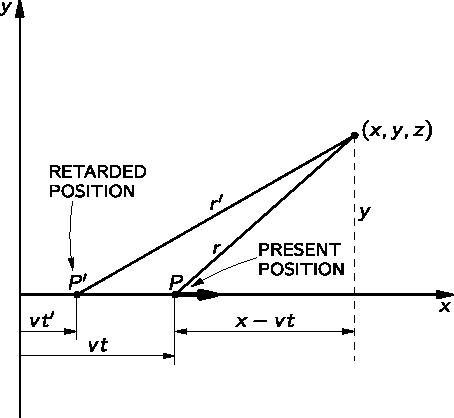
\includegraphics[width=0.7\linewidth]{fyz_fig0602.pdf}
      \caption{
               (\cite[s.~707]{Feynman02})}
      \label{fyz:fig0602}
    \end{figure}

    \begin{figure}[ht!] %\ref{fyz:fig0603}
      \centering
      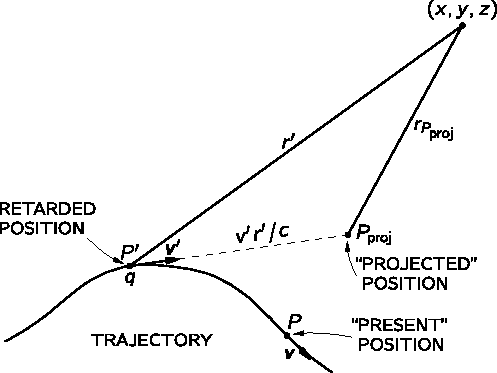
\includegraphics[width=0.7\linewidth]{fyz_fig0603.pdf}
      \caption{
               (\cite[s.~707]{Feynman02})}
      \label{fyz:fig0603}
    \end{figure}

    \begin{figure}[ht!] %\ref{fyz:fig0604}
      \centering
      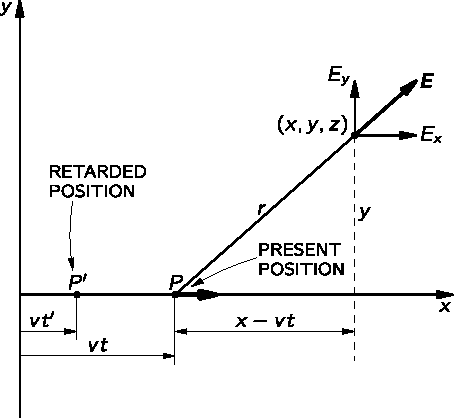
\includegraphics[width=0.7\linewidth]{fyz_fig0604.pdf}
      \caption{
               (\cite[s.~707]{Feynman02})}
      \label{fyz:fig0604}
    \end{figure}

    \begin{figure}[ht!] %\ref{fyz:fig0605}
      \centering
      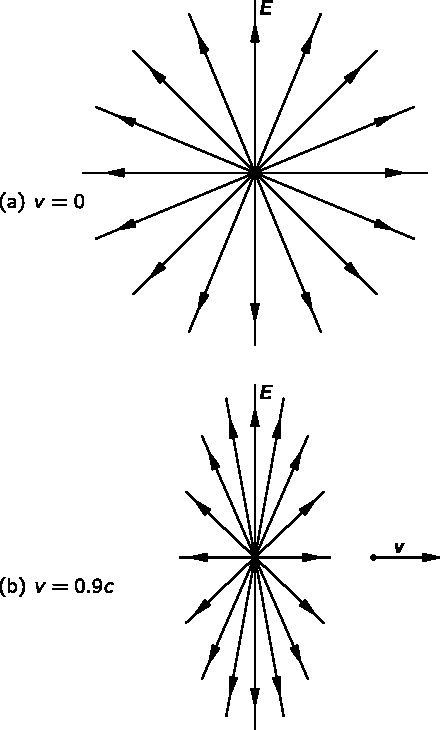
\includegraphics[width=0.7\linewidth]{fyz_fig0605.pdf}
      \caption{
               (\cite[s.~707]{Feynman02})}
      \label{fyz:fig0605}
    \end{figure}

    \begin{figure}[ht!] %\ref{fyz:fig0606}
      \centering
      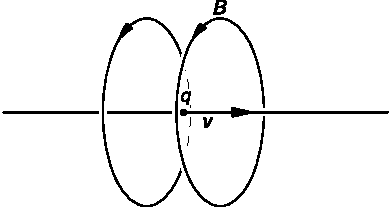
\includegraphics[width=0.7\linewidth]{fyz_fig0606.pdf}
      \caption{
               (\cite[s.~707]{Feynman02})}
      \label{fyz:fig0606}
    \end{figure}

    \begin{figure}[ht!] %\ref{fyz:fig0607}
      \centering
      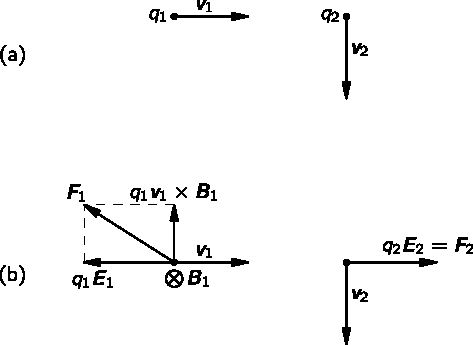
\includegraphics[width=0.7\linewidth]{fyz_fig0607.pdf}
      \caption{
               (\cite[s.~707]{Feynman02})}
      \label{fyz:fig0607}
    \end{figure}

    \begin{figure}[ht!] %\ref{fyz:fig0608}
      \centering
      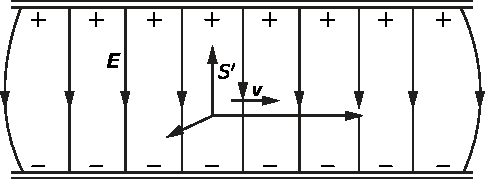
\includegraphics[width=0.7\linewidth]{fyz_fig0608.pdf}
      \caption{
               (\cite[s.~707]{Feynman02})}
      \label{fyz:fig0608}
    \end{figure}

    \todo[inline]{Kapitola fey2ch26 je nedodělaná, obsahuje pouze obrázky}
%} %tikzset
%---------------------------------------------------------------------------------------------------